\documentclass[letterpaper,12pt]{article}
\usepackage[utf8]{inputenc}
\usepackage{fullpage}
\usepackage{courier}
\usepackage[margin=0.75in]{geometry}
\usepackage{listings}
\usepackage{color}
\usepackage{graphicx}
\usepackage[width=5in]{caption}
\usepackage{hyphenat}
\usepackage{hyperref}
\usepackage{float}
\usepackage{multirow}

% Format a sectionless paragraph
\newcommand*\unparagraph{
	\par
	\nopagebreak
	\vskip3.25ex plus1ex minus.2ex
	\noindent
}

% define extra colors
\definecolor{dkgreen}{rgb}{0,0.6,0}
\definecolor{purple}{RGB}{159,0,197}

% define the code listing format
\lstset{
	language=C++,
	basicstyle=\footnotesize\ttfamily,
	backgroundcolor=\color{white},
	showspaces=false,
	showstringspaces=false,
	frame=none,
	tabsize=3,
	keywordstyle=\color{purple},
	commentstyle=\color{dkgreen},
	stringstyle=\color{blue},
	escapeinside={\%*}{*)}
}

% efine the title/header
\title{\Large CS 3468\\Lab 5} 
\author{Jared Wallace}
\date{}

\begin{document}

\maketitle

\vspace{30mm}

\section*{Objectives}
\begin{enumerate}
\item Build a sensor application that detects and locates mobile object
\item Understand the pro's and con's of teamwork
\end{enumerate}

\section*{Overview}
In this project, y'all will build a sensor network to track a mobile object
that carries a light. In the network, sensors will detect the object by sensing
the light. Because each sensor has a different distance to the light, the light
intensity recorded by each sensor will vary according to the distance from the source.
By collecting and analyzing all sensing data, the network will be able to detect and
locate the mobile object.

The network will look like the diagram below, where the triangle symbol represents the source
light, the circle symbols represent sensors and the square symbol represents the base station.
The base station will be what collects the data from the sensors and computes the location of
the source light.

Because the network area is large, sensors farther away from the base station will be unable to
communicate directly with the base station. Instead, their data must traverse other sensors in
order to reach the base station. The dashed lines represent how that data is forwarded through
other sensors to reach the base station.

\section*{Team}
This will be a whole class effort. Each student will have the responsibility of programming their
own sensor. You will be provided one local base station app for debugging purposes. When we build
the final network, one bad sensor node will break the network (there's the con of teamwork).

I will give you the following information:
\begin{itemize}
    \item The ID of the sensor
    \item The ID of the local base station (your personal debugging base station)
    \item The ID of the next hop
    \item The ID of the previous hop
\end{itemize}

\section*{Tasks}

\section*{Lab Report}
\begin{enumerate}
   \item Please demonstrate your program to the lab instructor and let him check your code at the end of the current lab project.
   \item Your project report is due at the beginning of the next lab.
   \item Grading criteria
      \begin{itemize}
         \item Demonstration, 15 percent
         \item Code, 15 percent
         \item Report, 70 percent
      \end{itemize}
\end{enumerate}
\section*{Report instructions}
Format:
\begin{enumerate}
   \item Include your name and ID in the first page
   \item Font size of at least 10pt
   \item Single spaced
   \item Maximum of 5 pages (I will take points off for exceeding this without any good reason)
   \item Please submit as PDF online, and turn in a hard copy
\end{enumerate}
Content:
\begin{enumerate}
   \item Introduction (10 percent of your grade) Please summarize the task of this lab and what you have learned in the lab
   \item Reset interrupt (20 percent of your grade) Please describe in detail how you designed
       and implemented part one. Make a diagram (you can draw this by hand and attach it) of the
       components you used and how they are wired. Make sure you include how you implemented the counter.
    \item UART (40 percent of your grade) Please describe in detail how you designed and implemented part
        two. Attach a diagram (as before, this may be hand drawn) showing the components you used and
        how they are wired. Show me the result of the command:
        \begin{lstlisting}
        java -jar serial.jar hdlc
        \end{lstlisting}
        Discuss what layers in the OSI model these results belong to, and what (if any) data is in the other layers of the OSI model.
\end{enumerate}

% Comic at the bottom
\begin{figure}[ht!]
	\centering
	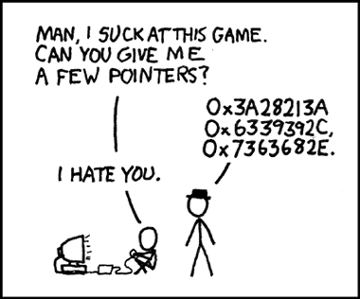
\includegraphics[width=4in]{pointers.png}
    \caption*{Every computer, at the unreachable memory address 0x-1, stores a secret.  I found it, and it is that all humans ar-- SEGMENTATION FAULT.}
\end{figure}

\end{document}
